%!TEX spellcheck=ro_RO
%!TEX root = ./main.tex
\chapter{Prezentarea aplicației}\label{ch:3implementare}

\textbf{Note implementare:}
\begin{enumerate}
\item Diferite incercari de a extrage feateruri
\item Probleme intampinate in asemanarea datelor NEUTRAL si RELAXED
\item Uita-te pe notebooku Licenta\_CNN
\end{enumerate}

Scopul lucrării îl constituie folosirea paradigmei învățării automate supervizate, mai precis, utilizarea rețelelor neuronale convoluționale pentru clasificarea a trei stări mentale diferite, și anume: \textit{neutru, relaxat} și \textit{concentrat}. 

Datele aferente fiecărei stări provin de la un dispozitiv comercial, \textit{Muse 2016}, capabil de a înregistra activitatea cerebrală folosind tehnica de imagistică \textit{EEG (Electroencefalografia)}, neinvazivă. Aceste înregistrări reprezintă activitatea creierului din jurul electrozilor dispusă în timp. Deoarece dispozitivul folosit folosește o tehnică neinvazivă cu electrozi uscați datele finale ale înregistrării conțin zgomot produs de mișcările persoanei, de contracțiile mușchilor sau chiar de clipit. Din aceste motive datele trebuie prelucrate. Este de menționat faptul că nu există o anumită formulă de prelucrare pentru ca datele sa fie perfecte pentru etapa de clasificare, metodele folosite în această etapă fiind stabilite adesea empiric. După prelucrarea datelor, urmează un pas de extragere a anumitor atribute/caracteristici statistice și spectrale pe baza cărora vor fi construite imaginile alb-negru. Fiecare imagine va avea o etichetă aferentă clasei din care face parte, neutru, relaxat sau concentrat.

După etapa de prelucrare și etichetare a datelor, urmează pregătirea datelor pentru transformarea acestora sub forma unor imagini alb-negru. Această etapă include selectarea celor mai relevante 400 de atribute, dintr-un total de 414. Pentru a putea fi folosite ca și componente ale unei imagini alb-negru, este necesară normalizarea datelor în intervalul $[0,1]$, 0 reprezentând negru, 1 reprezentând alb, orice altă valoare aparținând intervalului reprezentând o nuanță de gri. Imaginile sunt împărțite apoi în diferite seturi, fiecare cu scopul său specific; setul de antrenare, setul de validare și setul de testare. Antrenarea rețelei convoluționale se realizează folosind setul de antrenare și setul de validare pentru evaluarea performanțelor pe parcursul antrenării. În final, setul de testare este folosit pentru a determina performanța rețelei pe date complet noi, rezultând metricile finale, precum acuratețea sau valoarea funcției de cost \textit{(loss)}. În cazul rețelei dezvoltate în această lucrare a fost atinsă o acuratețe de $\approx91.83\%$ cu valoarea funcției de loss de $\approx0.2511$

În continuarea capitolului, etapele prezentate sumar anterior vor fi detaliate și explicate, urmând ca la finalul capitolului să fie prezentate rezultatele implementării.

\section{Etape implementare}

\subsection{Achiziție date}
Pentru achiziția datelor a fost folosită casca comercial valabilă Muse 2016. Aceasta conține cinci electrozi uscați, unul fiind folosit ca punct de referință, iar ceilalți patru pentru a înregistra semnalele EEG. Electrozii sunt poziționați în locațiile \textit{TP9, AF7, Fpz, AF8, TP10}, conform unei versiuni modificate a sistemului internațional 10-20 de poziționare al electrozilor EEG. Electrodul Fpz este folosit ca electrod de referință. În \autoref{fig:eegstandard} este prezentat aranjamentul electrozilor.

\begin{figure}[ht]
\centering
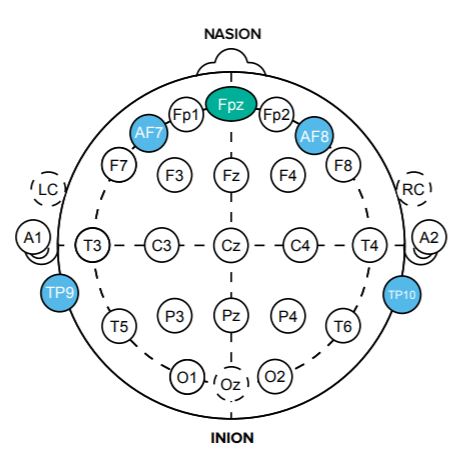
\includegraphics[width=10cm, keepaspectratio]{fig/cap3/EEGstandard.png}
\caption{Versiunea modificată a sistemului internațional 10-20 împreună cu marcajul poziției electrozilor căștii Muse \cite{online:muse-eeg}}
\label{fig:eegstandard}
\end{figure}

Pentru a diminua zgomotul înregistrat de senzori, pentru fiecare stare au fost alese activități care necesitau o mișcare minimă a persoanei examinate. Citirile datelor de la electrozii AF7 și AF8, fiind situați pe frunte, sunt distorsionate de mișcările generate de clipit. Astfel, pentru a păstra o uniformitate asupra celor trei stări, clipitul nu a fost nici încurajat nici descurajat. Chiar dacă acesta este considerat zgomot, rata de clipire este influențată de starea de concentrare a persoanei, acest lucru fiind util în final pentru algoritmul de clasificare. Totuși, persoanelor examinate le-a fost specificat să nu inchidă ochii pe durata unui test.

Pentru determinarea celor trei stări mentale, au fost stabilite trei activități, conform \cite{eeg:2018}. Pentru înregistrarea stării neutre, participanții au fost îndrumați să păstreze o poziție confortabilă a corpului și o stare mentală echilibrată, nici prea relaxată dar nici prea activă. Înregistrarea stării mentale de relaxare a presupus ca subiecții să asculte o piesă muzicală cu o tonalitate și un tempo scăzut. Acestora le-a fost indicat faptul de a se relaxa complet, atât fizic cât și psihic. Pentru determinarea stării mentale active și concentrate participanții au fost instruiți să joace o variantă a jocului „alba-neagra”, în care un obiect este ascuns sub unul din mai multe pahare, care mai apoi sunt amestecate între ele. Scopul jocului fiind de a identifica paharul care conține obiectul. Pe parcursul jocului, numărul paharelor și viteza cu care acestea se mișcă va crește.

Activitățile au fost desfășurate începând cu starea neutră, urmată de starea de relaxare, iar la final starea de concentrare. Pentru fiecare activitate în parte au fost efectuate două înregistrări ale datelor EEG pe o durată de 65 de secunde. Primele 3 și ultimele 2 secunde fiind șterse ulterior, scopul acestora fiind de a crea o zonă de tranziție. A mai fost observată și o transmisie cu frecvență variabilă ($\approx256\si{\hertz}$) a datelor de către casca Muse, astfel zonele de tranziție ajutând la uniformizarea datelor. Datele EEG au fost colectate de la 12 persoane, 5 de sex feminin, 7 de sex masculin. În total au fost înregistrate 26 de minute per stare, din care 24 de minute utilizabile. În \autoref{fig:muse_eeg_sample} pot fi observate semnalele provenite de la fiecare electrod în parte. Casca oferă posibilitatea de a adăuga un senzor în plus, semnalul acestuia fiind transmis prin canalul RightAUX. Semnalul provenit de la canalul în cauză a fost eliminat deoarece nu avea conectat un senzor, transmițând astfel doar zgomot.

\begin{figure}[ht]
\centering
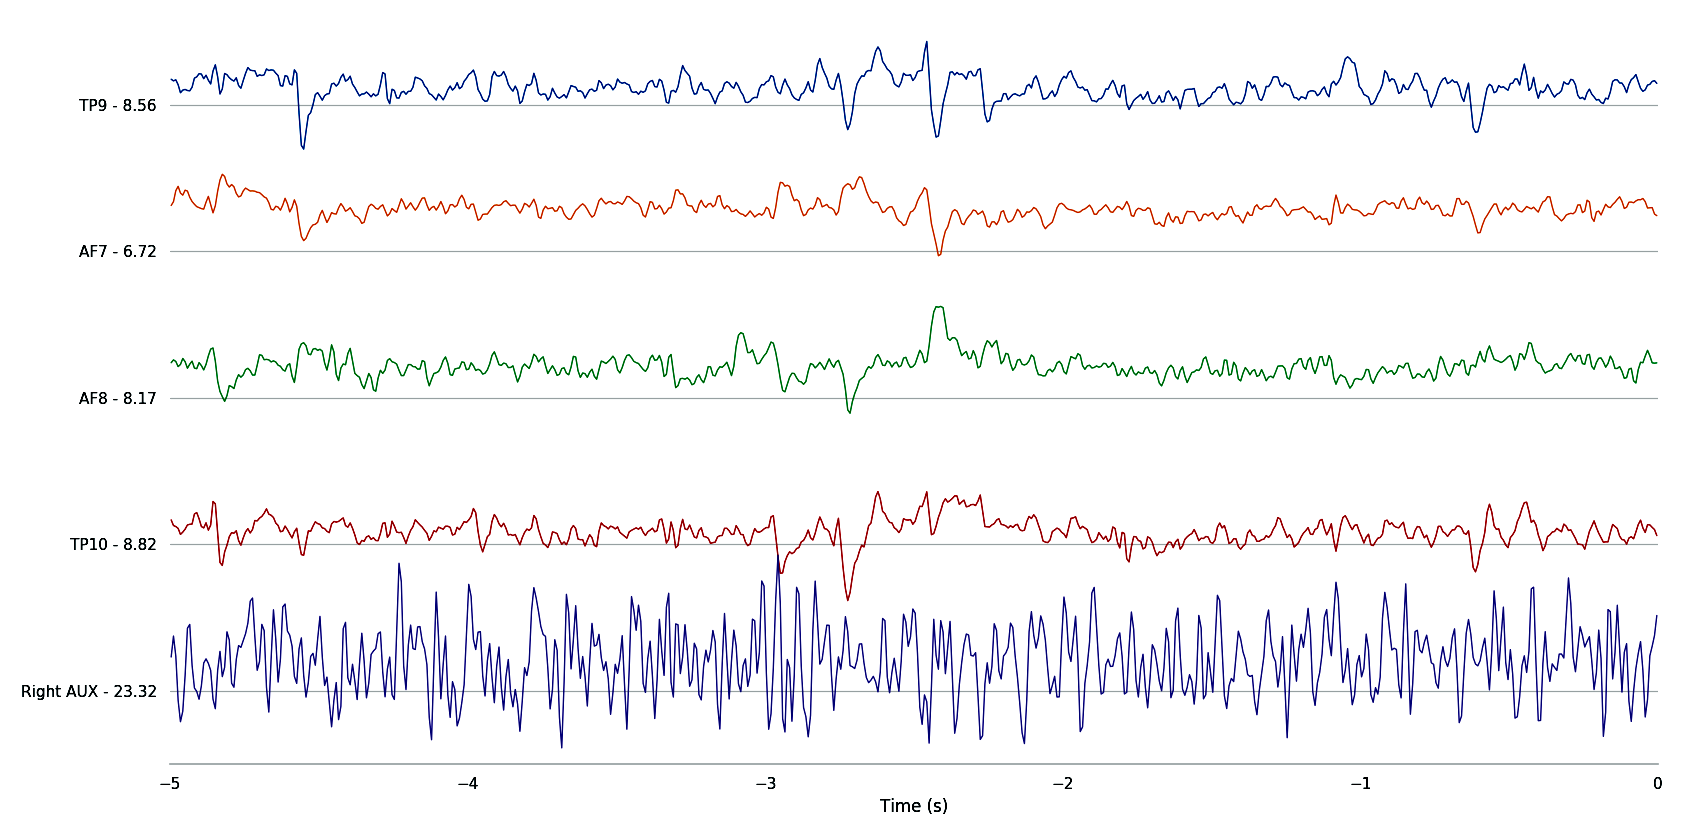
\includegraphics[width=\textwidth, keepaspectratio]{fig/cap3/museEEGplot.png}
\caption{Exemplu semnale EEG Muse 2016, extrase folosind librăria MuseLSL \cite{online:muselsl}}
\label{fig:muse_eeg_sample}
\end{figure}

\subsection{Extragerea atributelor}
Etapa de extragere a atributelor are rolul de a crea un set de date bazat pe semnalele EEG înregistrate, cu scopul de a fi cât mai informative pentru scopul algoritmului. Astfel, se elimină informația redundantă și nesemnificativă obiectivului, aducând avantaje precum scăderea timpului de învățăre a rețelei și o mai bună generalizare a datelor. În această lucrare, setul de date format din atribute ale semnalului EEG, este alcătuit din două seturi de date formate din atribute statistice respectiv atribute spectrale. Tipurile de atribute extrase, atât cele statistice cât și cele spectrale, au fost influențate de către lucrările \cite{eeg-cnn:2020} și \cite{eeg:2018}.

Pentru calculul atributelor, semnalul a fost împărțit în „ferestre”, notate $w_i$, conținând un set de $N$ valori ale semnalului pentru durata de 1 secundă, transmise cu frecvența $256\si{\hertz}$. Ferestrele conțin o suprapunere de 0.5 secunde, astfel $w_1=[0,1]$, $w_2=[0.5,1.5]$, $w_3=[1,2]$, etc. Din fiecare fereastră rezultată au mai fost create, prin împărțirea fiecărei ferestre $w_i$, jumătăți și sferturi de fereastră. Rezultând astfel $w_{h1}$ și $w_{h2}$, reprezentând prima respectiv a doua jumătate a ferestrei, fiecare conținând $N/2$ valori, iar $w_{q1}$, $w_{q2}$, $w_{q3}$, $w_{q4}$ reprezentând sferturile ferestrei, fiecare conținând $N/4$ valori.

\subsubsection*{Atribute statistice}
Având aceste ferestre create, pentru fiecare fereastră $w_i$ au fost extrase atribute statistice considerând fie întreaga fereastră, fie jumătățile, fie sferturile. Astfel, pentru fiecare semnal EEG, au fost extrase următoarele atribute:
\begin{itemize}
	\item Considerând o întreagă fereastra, $w$:
	\begin{enumerate}
	\item Media valorilor ferestrei
	\begin{equation}
	\mu = \frac{1}{N}\sum_n^N x_n
	\end{equation}
	unde $x_n$ reprezintă setul de valori dintr-o fereastră
	\item Deviația standard a valorilor
	\begin{equation}
	\sigma = \sqrt{\frac{1}{N}\sum_n^N(x_n - \mu)^2}
	\end{equation}
	\item Varianța (dispersia) valorilor
	\begin{equation}
	\sigma^2 = \frac{1}{N}\sum_n^N(x_n - \mu)^2
	\end{equation}
	\item Momentul centrat de ordin 3 (asimetria valorilor) 
	\begin{equation}
	\mu_3 = \frac{1}{N}\sum_n^N(x_n - \mu)^3
	\end{equation}
	\item Momentul centrat de ordin 4 (aplatizarea valorilor)
	\begin{equation}
	\mu_4 = \frac{1}{N}\sum_n^N(x_n - \mu)^4
	\end{equation}
	\item Covarianța perechilor de semnale EEG (TP9, AF7, AF8, TP10)
	\begin{equation}
	cov(X,Y) = \frac{1}{N}\sum_n^N(x_n - \bar{x})(y_n - \bar{y})
	\end{equation}
	unde $x_n$ și $y_n$ reprezintă setul de valori dintr-o fereastră a unui semnal EEG, iar $\bar{x}$ și $\bar{y}$ reprezintă media acestora
	\item Valoarea maximă și valoarea minimă a ferestrei
	\end{enumerate}
	\item Considerând jumătățile de fereastră, $w_{h1}$ și $w_{h2}$:
	\begin{enumerate}
		\item Diferența dintre media valorilor jumătăților
		\item Diferența dintre deviația standard a valorilor jumătăților
		\item Diferența dintre maximul valorilor jumătăților
		\item Diferența dintre minimul valorilor jumătăților
	\end{enumerate}
	\item Considerând sferturile de fereastră, $w_{q1}$, $w_{q2}$, $w_{q3}$, $w_{q4}$:
		\begin{enumerate}
		\item Media valorilor sferturilor de fereastră
		\item Diferența mediilor perechilor de ferestre
		\item Valoarea maximă și valoarea minimă a ferestrelor
		\item Diferența maximelor perechilor de ferestre
		\item Diferența minimelor perechilor de ferestre
	\end{enumerate}
\end{itemize}

La final, a rezultat un total de 174 de atribute statistice.

\subsubsection*{Atribute spectrale}
Comparativ cu atributele statistice, generarea atributelor spectrale a fost făcută doar pe ferestre întregi, $w_i$. În cadrul extragerii atributelor spectrale a fost efectuată o prelucrare a semnalului înainte de a calcula atributele. Inițial, a fost realizată o centrare a întregului semnalului în jurul valorii $0$, iar mai apoi a fost aplicat un filtru trece-jos de tip Chebyshev I (Fig. \ref{fig:cheb1-filt}), cu frecvența de tăiere de $50\si{\hertz}$. Prin această filtrare se păstrează doar banda de frecvență relevantă undelor cerebrale, și anume $1-50\si{\hertz}$.
\begin{figure}[ht]
\centering
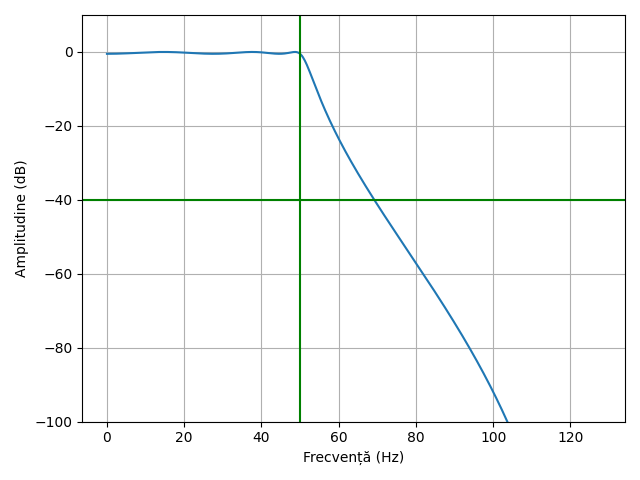
\includegraphics[width=\textwidth, keepaspectratio]{fig/cap3/cheb1-filt.png}
\caption{Răspunsul în frecvența a filtrului trece-jos de tip Chebyshev I de ordin 6}
\label{fig:cheb1-filt}
\end{figure}

După aplicarea filtrului asupra întregului semnal EEG, a fost calculată Transformata Fourier Discretă \textit{(DFT)}, folosind algoritmul \textit{Fast Fourier Transform (FFT)}. Apoi au fost extrase amplitudinile fiecărei componente ale semnalului filtrat, rezultând 50 de atribute per semnal. Ultimele atribute extrase au fost amplitudinile celor mai puternice 10 frecvențe din componența semnalului. În total, au rezultat 260 de atribute.

Combinând cele 174 de atribute statistice cu aceste 260 de atribute spectrale, rezultă un total de 414 atribute. În setul de date format din acestea, se adaugă și clasa fiecărei înregistrări.

\subsection{Arhitectura rețelei}

\subsection{Antrenarea rețelei}

\subsection{Evaluarea și ajustarea parametrilor}

\section{Rezultate}
